% $Header$

\documentclass{beamer}

% This file is a solution template for:

% - Giving a talk on some subject.
% - The talk is between 15min and 45min long.
% - Style is ornate.



% Copyright 2004 by Till Tantau <tantau@users.sourceforge.net>.
%
% In principle, this file can be redistributed and/or modified under
% the terms of the GNU Public License, version 2.
%
% However, this file is supposed to be a template to be modified
% for your own needs. For this reason, if you use this file as a
% template and not specifically distribute it as part of a another
% package/program, I grant the extra permission to freely copy and
% modify this file as you see fit and even to delete this copyright
% notice.


\mode<presentation>
{
%  \usetheme{Warsaw}
  % or ...

  \setbeamercovered{transparent}
  % or whatever (possibly just delete it)
}


\usepackage[english]{babel}
% or whatever

\usepackage[latin1]{inputenc}
% or whatever

\usepackage{times}
\usepackage[T1]{fontenc}
% Or whatever. Note that the encoding and the font should match. If T1
% does not look nice, try deleting the line with the fontenc.

\usepackage{graphicx}

\title{Memristors}
\author{Charles Pittman}
\institute{The Citadel\\ELEC-424}
% - Keep it simple, no one is interested in your street address.

\date{\today}

% If you have a file called "university-logo-filename.xxx", where xxx
% is a graphic format that can be processed by latex or pdflatex,
% resp., then you can add a logo as follows:

 \pgfdeclareimage[height=0.5cm]{university-logo}{university-logo.jpg}
 \logo{\pgfuseimage{university-logo}}



% Delete this, if you do not want the table of contents to pop up at
% the beginning of each subsection:
%\AtBeginSubsection[]
%{
%  \begin{frame}<beamer>{Outline}
%    \tableofcontents[currentsection,currentsubsection]
%  \end{frame}
%}


% If you wish to uncover everything in a step-wise fashion, uncomment
% the following command:

%\beamerdefaultoverlayspecification{<+->}


\begin{document}

\begin{frame}
  \titlepage
\end{frame}

\begin{frame}{Outline}
  \tableofcontents
  % You might wish to add the option [pausesections]
\end{frame}


% Since this a solution template for a generic talk, very little can
% be said about how it should be structured. However, the talk length
% of between 15min and 45min and the theme suggest that you stick to
% the following rules:

% - Exactly two or three sections (other than the summary).
% - At *most* three subsections per section.
% - Talk about 30s to 2min per frame. So there should be between about
%   15 and 30 frames, all told.

\section{Introduction}

\subsection{What is it?}

\begin{frame}{Make Titles Informative. Use Uppercase Letters.}{Subtitles are optional.}
  % - A title should summarize the slide in an understandable fashion
  %   for anyone who does not follow everything on the slide itself.

  \begin{itemize}
  \item
    Use \texttt{itemize} a lot.
  \item
    Use very short sentences or short phrases.
  \end{itemize}
\end{frame}

\begin{frame}{Make Titles Informative.}

  You can create overlays\dots
  \begin{itemize}
  \item using the \texttt{pause} command:
    \begin{itemize}
    \item
      First item.
      \pause
    \item
      Second item.
    \end{itemize}
  \item
    using overlay specifications:
    \begin{itemize}
    \item<3->
      First item.
    \item<4->
      Second item.
    \end{itemize}
  \item
    using the general \texttt{uncover} command:
    \begin{itemize}
      \uncover<5->{\item
        First item.}
      \uncover<6->{\item
        Second item.}
    \end{itemize}
  \end{itemize}
\end{frame}

\begin{frame}
  \center
  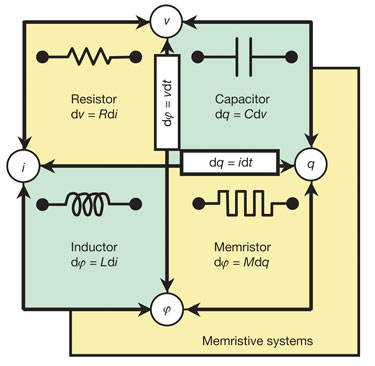
\includegraphics[height=7cm]{memristor02.jpg}
\end{frame}

\begin{frame}
  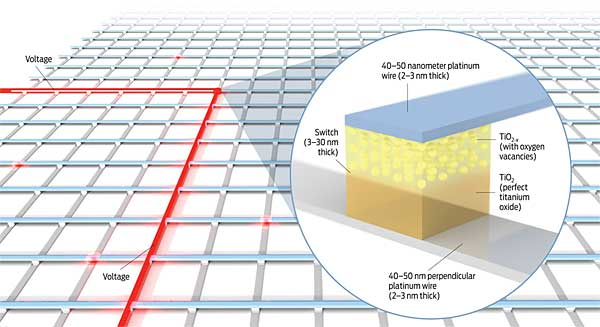
\includegraphics[height=6cm]{memristor01.jpg}
\end{frame}

\subsection{How does it work?}

\begin{frame}
\end{frame}

\begin{frame}
\end{frame}

\section{Applications}

\subsection{Non-Volatile Memory}
\begin{frame}{Non-Volatile Memory}

\end{frame}
\subsection{Logic}
\begin{frame}{Logic}
\begin{table}[h]
\centering
\caption{IMPLY}
\begin{tabular}{cc|c}
P & Q & P $\Rightarrow$ Q \\
\hline
1 & 1 & 1 \\
1 & 0 & 0 \\
0 & 1 & 1 \\
0 & 0 & 1
\end{tabular}
\end{table}
\end{frame}
\subsection{Learning Circuits}
\begin{frame}{Learning Circuits}

\end{frame}

\section*{Summary}

\begin{frame}{Summary}

  % Keep the summary *very short*.
  \begin{itemize}
  \item
    The \alert{first main message} of your talk in one or two lines.
  \item
    The \alert{second main message} of your talk in one or two lines.
  \item
    Perhaps a \alert{third message}, but not more than that.
  \end{itemize}

  % The following outlook is optional.
  \vskip0pt plus.5fill
  \begin{itemize}
  \item
    Outlook
    \begin{itemize}
    \item
      Something you haven't solved.
    \item
      Something else you haven't solved.
    \end{itemize}
  \end{itemize}
\end{frame}

\end{document}

\author{Charles Pittman}
\date{\today}
\title{Memristors}

\documentclass[12pt]{article}

\begin{document}
\maketitle

%\begin{abstract}
%This is the paper's abstract \ldots
%\end{abstract}

\section{Introduction}
Electronics textbooks list three passive components: resistors, capacitors, and
inductors.  Resistors relate voltage to current, capacitors relate voltage to
charge, and inductors relate charge to magnetic flux.  Noting the symmetry (no
component relating magnetic flux to current), in 1971 Leon Chua published a
mathematical proof \cite{chua1971} that such a device should be possible.

As a function of time, the device gives a flux-charge relationship similar to
the current-voltage relationship of a resistor (i.e. its resistance changes
according to the charge passed through it).  The device remembers it's history,
which is where the term ``memristor'' comes from.  Active devices simulating
the behavior had existed, but the first passive version came from HP 37 years
later. \cite{strukov2008missing}

%\section{Implementation}
%\subsection{Titanium Dioxide}
HP's device consisted of two layers of titanium dioxide ($\mathrm{TiO_2}$), a
semiconductor, sandwiched between platinum plates with some oxygen atoms
removed from one of the layers to make it conductive ($\mathrm{TiO_{2-x}}$).
Voltage applied to the platinum plates would expand or contract the
$\mathrm{TiO_{2-x}}$ layer, changing the device's conductivity
\cite{williams2008we} (a switch, essentially).

\section{Applications}


\subsection{Non-Volatile Memory}\label{memory}
The device HP created was born out of a research group tasked with figuring out
what to do when transistors could be shrunk no further \cite{williams2008we}.
As component sizes shrink aligning masks during the die creation becomes more
difficult and probability of surface defects increase, together reducing yield
\cite{snider2008molecular}.  The team realized that redundancy could be used to
combat the reduced yield.  Inspired by another HP project, the Teramac
\cite{heath1998} massively-parallel computer, the cross-board latch would be
used: multiple switches are placed between an input and output line such that
any could trigger a connection.  Forming an array of these latches created a
storage device, and since memristors preserve their state no power is required
to preserve the data.

\subsection{Logic}\label{logic}
The extension from storage to logic is straightforward: for any operation a
given input will produce the same output, so a table of results can be created
for a list of inputs.  Memristors can implement logic functions as well; the
basic NAND gate requires one less component compared to transistors.  Besides
boolean logic memristors can be used to build the IMPLY conditional (p
$\Rightarrow $ q) \cite{DBLP:journals/corr/abs-1110-2074} which is useful in implementing fuzzy logic.

\subsection{Learning Circuits}\label{ai}
A 2009 study\cite{pershin2009} showed a simple memristive circuit was able to
anticipate voltage spikes when a steady pulse train was applied.  The
experiment was designed to emulate an earlier study \cite{saigusa2008} on
behavioral intelligence in slime mold.  In it the mold was able to predict
periodic changes to its environment.  A separate study
\cite{nakagaki2000intelligence} of the slime mold showed the single-cell
organisms capable of solving a maze via the shortest path; a network of memristors was later shown capable of the same \cite{pershin2011}.

%\subsection{Base-n Memory}
%In 2014 physicists at Trinity College Dublin created a memristor able to switch
%to six discrete states. \cite{hellemans_2014}

\newpage{}

\bibliographystyle{abbrv}
\bibliography{main}

\end{document}
This is never printed
